\documentclass[10pt,aspectratio=169]{beamer}
\usepackage[utf8]{inputenc}
\usepackage[T1]{fontenc}
\usepackage{graphicx}
\usepackage{booktabs}
\usepackage{multirow}
\usepackage{amsmath}
\usepackage{amssymb}

\usetheme{Madrid}
\usecolortheme{seahorse}

\title{Multi-Agent Price Discovery}
\subtitle{Analytical HJB vs PPO HJB Market Makers in a Kyle-Style Informed Market}
\author{Team}
\date{\today}

\begin{document}

% =====================================================================
% TITLE
% =====================================================================
\begin{frame}
  \titlepage
\end{frame}

% =====================================================================
\section{MARL Environment}
% =====================================================================

\begin{frame}{MARL Simulation Environment: Architecture}
  \begin{columns}[T]
    \column{0.55\textwidth}
    \textbf{Core design:}
    \begin{itemize}
      \item Rust-backed limit-order-book exchange (\texttt{\_sim\_exchange})
      \item Python agent lifecycle: each agent implements \texttt{on\_tick()}
      \item The loop is \textbf{agent-agnostic}: advances time, calls \texttt{on\_tick} on every agent, collects nothing
      \item Agents self-log their own CSV metrics
    \end{itemize}

    \vspace{6pt}
    \textbf{Execution per tick:}
    \begin{enumerate}
      \item Market ticks forward ($\Delta t = 1$)
      \item Each agent's \texttt{on\_tick()} runs and \textbf{blocks} until it returns
      \item Market state updates from order executions
      \item Repeat
    \end{enumerate}

    \column{0.45\textwidth}
    \centering
    \vspace{20pt}
    \texttt{\footnotesize
    for tick in range(n\_ticks): \\
    \quad market.tick() \\
    \quad for agent in agents: \\
    \quad \quad agent.on\_tick(sim\_t) \\
    \quad sim\_t += 1
    }
  \end{columns}
\end{frame}

\begin{frame}{Agent Lifecycle \& Information Flow}
  \textbf{Each agent's \texttt{on\_tick()} follows the same pattern:}

  \vspace{6pt}
  \begin{enumerate}
    \item \textbf{Check scheduler:} if it is not this agent's decision time, return immediately
    \item \textbf{Drain acks/fills:} process confirmations and fills from the exchange since the last tick
    \item \textbf{Read market data:} \texttt{md = market.get\_md(asset\_id)} -- best bid/ask, full LOB, fill counters
    \item \textbf{Build observation:} agent-specific function that maps raw market data to a fixed-dimension state vector
    \item \textbf{Decide action:} sample from PPO policy (training) or deterministic forward pass (eval)
    \item \textbf{Submit orders:} \texttt{action\_to\_orders()} produces limit/market orders, sent through the agent's connection
    \item \textbf{Advance step counter:} increment internal decision step
  \end{enumerate}

  \vspace{6pt}
  \textbf{All orders} from all agents are collected by an \texttt{OrderShuffler}, interleaved randomly, then dispatched to the exchange in a single batch per tick.
\end{frame}

\begin{frame}{Order Routing and Market Data}
  \begin{columns}[T]
    \column{0.55\textwidth}
    \textbf{Order flow:}
    \begin{itemize}
      \item Independent agents (HJB MM, PPO HJB MM, IT) each have their own \texttt{conn} to the exchange
      \item The \texttt{OrderShuffler} meta-agent wraps sub-agents (UniformMMs, Poisson noise) and collects orders from independent agents
      \item All orders are pooled into one list, \texttt{random.shuffle()} is applied, then each order is dispatched through its originating agent's \texttt{conn}
      \item This prevents any agent from consistently getting priority at the exchange
    \end{itemize}

    \column{0.45\textwidth}
    \textbf{Market data returned by \texttt{get\_md()}:}
    \begin{itemize}
      \item \texttt{bid}, \texttt{ask} -- best bid/ask prices
      \item \texttt{bids[N]}, \texttt{asks[N]} -- LOB depth (price, volume)
      \item \texttt{taker\_volume\_buy/sell} -- cumulative market order volume
      \item \texttt{informed} -- direct informed-flow indicator (when available)
      \item Side-entry counters (nlab, nmb, nlas, nms)
    \end{itemize}
  \end{columns}
\end{frame}

\begin{frame}{PPO Training Lifecycle}
  \textbf{Each trainable agent runs its own PPO loop independently:}

  \vspace{6pt}
  \begin{columns}[T]
    \column{0.48\textwidth}
    \textbf{Within a rollout:}
    \begin{itemize}
      \item Collect $n$ steps (default $n = 40$)
      \item At each step: observation $\rightarrow$ action $\rightarrow$ reward $\rightarrow$ next observation
      \item Store transition in rollout buffer: $(s_t, a_t, r_t, s_{t+1})$
    \end{itemize}

    \vspace{4pt}
    \textbf{At buffer full (every $n$ steps):}
    \begin{enumerate}
      \item Compute advantages via GAE($\lambda$)
      \item Run PPO update ($K$ epochs, mini-batch SGD)
      \item Clear buffer, increment episode counter
      \item Call \texttt{on\_episode\_start()} to reset episode state
    \end{enumerate}

    \column{0.48\textwidth}
    \textbf{During the simulation:}
    \begin{itemize}
      \item \texttt{total\_timesteps} budget (default $20\,000$)
      \item Eval interleaving every \texttt{eval\_freq} steps
      \item Checkpointing every \texttt{checkpoint\_freq} steps
      \item Agents are completely independent -- they do not share parameters, buffers, or rewards
    \end{itemize}
  \end{columns}
\end{frame}

% =====================================================================
\section{Motivation \& Background}
% =====================================================================

\begin{frame}{What Are We Trying to Do?}
  \textbf{Goal:} Study price discovery in a limit-order-book market where:
  \begin{itemize}
    \item An \textbf{informed trader} (IT) knows the true fundamental value $v$ and exploits it
    \item \textbf{Market makers} provide liquidity but face adverse selection risk
    \item We compare three MM configurations: (1) fixed analytical HJB MMs only,
          (2) learned PPO HJB MMs only, (3) both together
    \item IT is trained separately in each environment
  \end{itemize}

  \vspace{6pt}
  \textbf{Key question:} Does a learned maker (PPO HJB) behave differently from an analytical one?
  Does coexistence change price discovery dynamics?
\end{frame}

\begin{frame}{The Kyle-Style Informed Model}
  \textbf{Classic Kyle (1985):}
  \begin{itemize}
    \item Single informed trader, market makers, noise traders
    \item IT trades on private information, MMs set prices
    \item Equilibrium: MM learns $\lambda$ (price impact), IT chooses order size
  \end{itemize}

  \vspace{6pt}
  \textbf{Our extension:}
  \begin{itemize}
    \item Discrete-time tick-by-tick simulation ($\Delta t = 1$)
    \item IT action: $\beta \in [0,10]$ linear policy \\
          $q = \beta \cdot (v - a_t)$
    \item IT reward: $(v - \text{fill price}) \cdot \text{volume}$
    \item IT is \texttt{buy\_only} (only exploits positive mispricing)
  \end{itemize}
\end{frame}

\begin{frame}{Market Maker Models}
  \textbf{Both MM types use the Gu\'eant HJB framework:}
  \begin{itemize}
    \item Solves a PDE backward on inventory grid $q \in [-20, 20]$
    \item Depth formula: $\delta_{\text{bid}} = \frac{1}{\kappa} + h(q) - h(q+1)$
    \item $\kappa$ controls fill-probability decay per tick
    \item Running penalty $\phi$ and terminal penalty $\alpha$ on $q^2$
  \end{itemize}

  \vspace{8pt}
  \begin{columns}[T]
    \column{0.50\textwidth}
    \textbf{Analytical HJB MM (fixed)}
    \begin{itemize}
      \item $\kappa = 0.8$, constant throughout
      \item $\lambda = 1.0$, fixed arrival rate
      \item No learning: quotes deterministically from PDE
    \end{itemize}

    \column{0.50\textwidth}
    \textbf{PPO HJB MM (trainable)}
    \begin{itemize}
      \item Learns $\kappa_t \in [0.01, 2.0]$ via PPO
      \item 7-dim observation: $q$, spread, $\lambda$ est., mid vol, imbalance, $t$, $\kappa_{t-1}$
      \item Reward: $\Delta\text{cash} - \phi q^2 \Delta t - \alpha q^2\cdot\mathbf{1}_{\text{last step}}$
      \item HJB PDE solved once at init with $\kappa_{\text{ref}} = 0.8$
    \end{itemize}
  \end{columns}
\end{frame}

\begin{frame}{The Market Environment}
  \begin{itemize}
    \item Reference price: $1000$, tick size: $1$, lot size: $1$
    \item Decision interval: $\Delta t = 1.0$, episode length: $40$ steps
    \item Training: $20\,000$ total timesteps, $40$ steps per rollout
    \item Evaluation: $30$ independent episodes (seeds $10\,000+$ep)
    \item Rust-backed exchange (\texttt{\_sim\_exchange}), agents interleaved via \texttt{OrderShuffler}
  \end{itemize}

  \vspace{8pt}
  \begin{center}
  \begin{tabular}{lll}
    \toprule
    Agent & Role & Parameters \\
    \midrule
    Poisson Noise & Random market orders & $\lambda^\pm = 1.0$ \\
    HJB MM ($\times 3$ or $\times 5$) & Fixed liquidity & $\kappa = 0.8$, $q \in [-20,20]$ \\
    PPO HJB MM ($\times 3$ or $\times 5$) & Learned liquidity & $\kappa \in [0.01, 2.0]$, $q \in [-20,20]$ \\
    Kyle Informed Trader & Directional flow & $\beta \in [0, 10]$, linear, buy-only \\
    \bottomrule
  \end{tabular}
  \end{center}
\end{frame}

% =====================================================================
\section{Experiment Configurations}
% =====================================================================

\begin{frame}{Six Experiments}
  \begin{center}
  \begin{tabular}{llcc}
    \toprule
    Fair Value $v$ & Configuration & HJB MMs & PPO HJB MMs \\
    \midrule
    \multirow{3}{*}{$v = 1003$\;(3 ticks above ref)} &
      HJB-only & 5 & 0 \\
    & PPO-only & 0 & 5 \\
    & Mixed (3+3) & 3 & 3 \\
    \midrule
    \multirow{3}{*}{$v = 1006$\;(6 ticks above ref)} &
      HJB-only & 5 & 0 \\
    & PPO-only & 0 & 5 \\
    & Mixed (3+3) & 3 & 3 \\
    \bottomrule
  \end{tabular}
  \end{center}
\end{frame}

% =====================================================================
\section{Results -- LOB Price Convergence}
% =====================================================================

\begin{frame}{$v = 1003$ -- HJB-Only (IT vs 5 analytical HJB MMs)}
  \begin{columns}[T]
    \column{0.62\textwidth}
    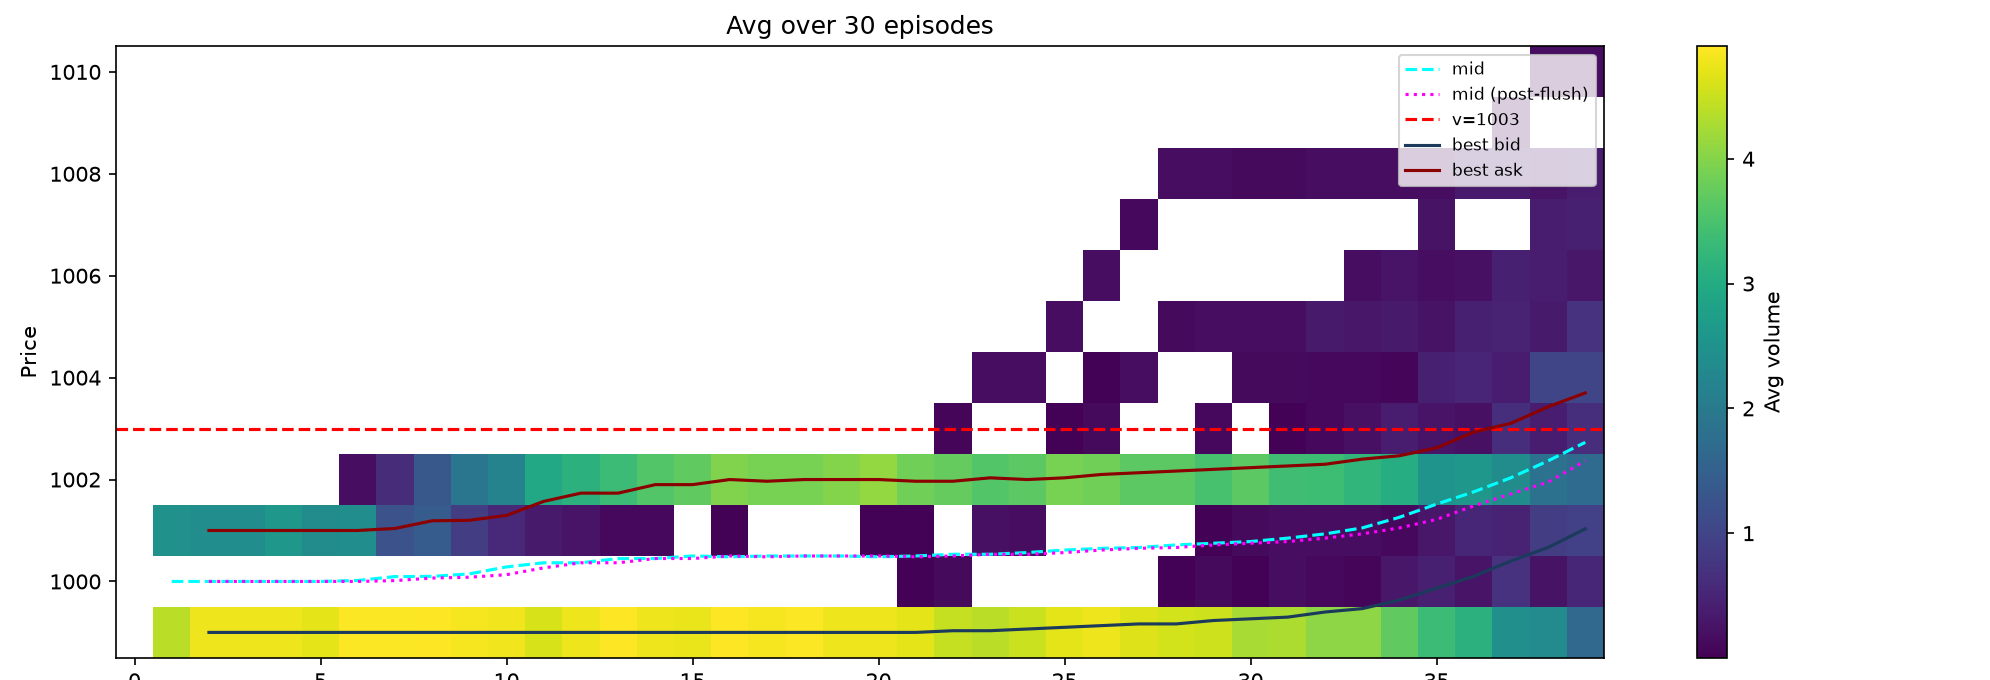
\includegraphics[width=\textwidth]{cropped/v1003_hjb_lob.png}
    \column{0.35\textwidth}
    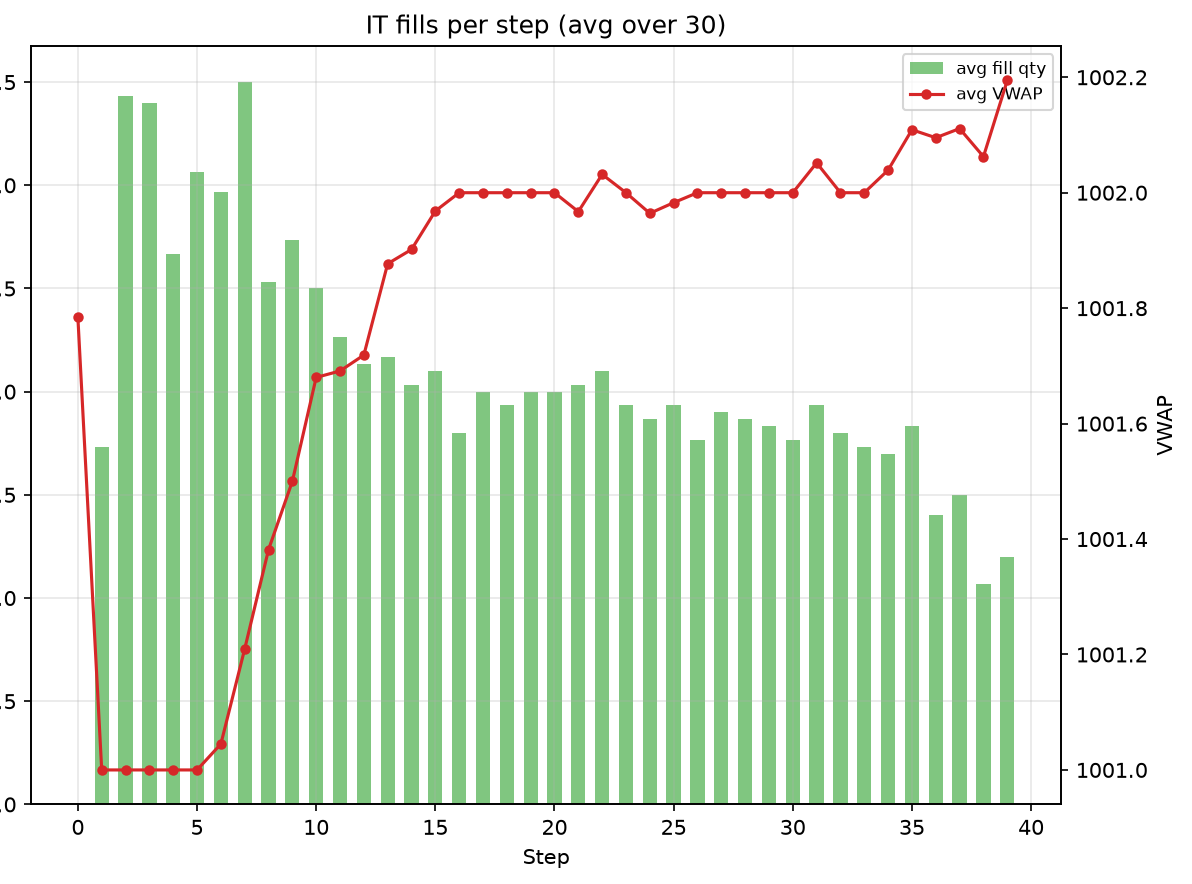
\includegraphics[width=\textwidth]{cropped/v1003_hjb_fills.png}
  \end{columns}
  \begin{itemize}
    \item Mid price converges smoothly toward $v = 1003$ ($\approx 1002.5$ by step 40)
    \item IT accumulates $\approx 20$--$25$ lots; IT's $\beta$ stays moderate ($\approx 2$--$3$)
    \item MM PnL positive -- they buy from noise, sell to IT at a mark-up
  \end{itemize}
\end{frame}

\begin{frame}{$v = 1003$ -- PPO-Only (IT vs 5 PPO HJB MMs)}
  \begin{columns}[T]
    \column{0.62\textwidth}
    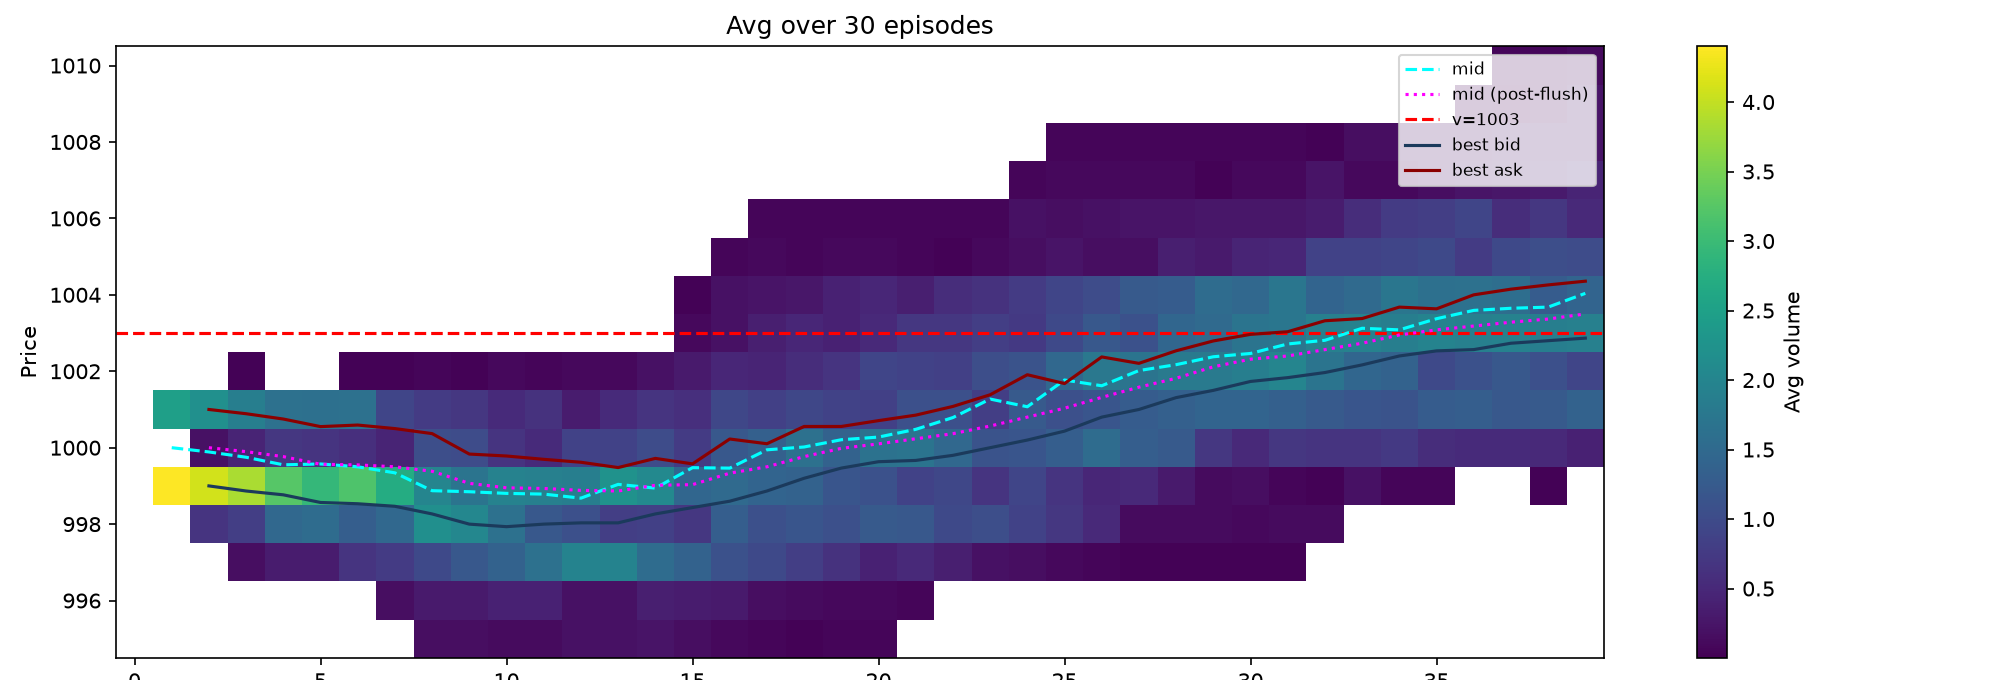
\includegraphics[width=\textwidth]{cropped/v1003_ppo_lob.png}
    \column{0.35\textwidth}
    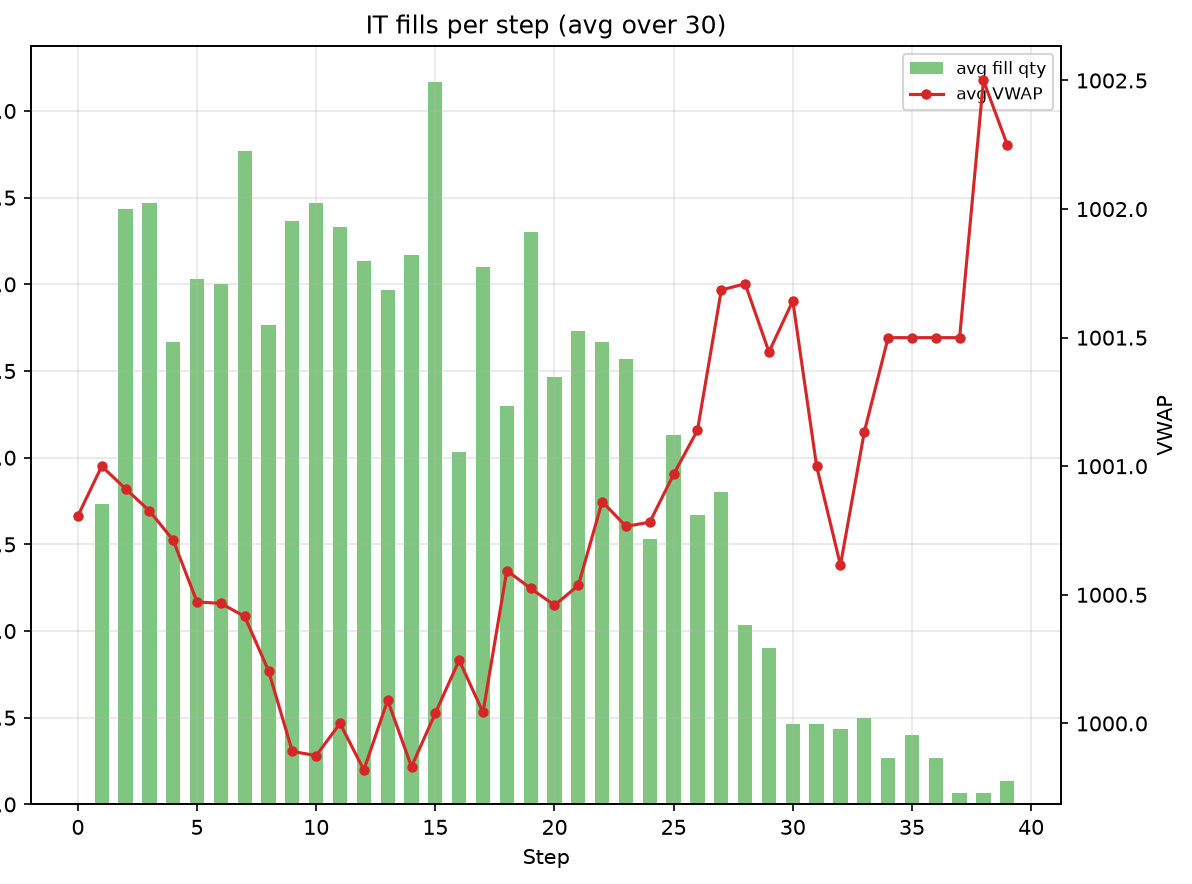
\includegraphics[width=\textwidth]{cropped/v1003_ppo_fills.png}
  \end{columns}
  \begin{itemize}
    \item \textbf{Dip-then-rise pattern}: mid drops to $\sim 997$ then climbs toward $1003$
    \item $\kappa$ starts $\sim 1.15$, dips to $\sim 1.07$, then rises to $\sim 1.32$
    \item PPO MMs widen spreads initially in response to informed flow, then tighten
  \end{itemize}
\end{frame}

\begin{frame}{$v = 1003$ -- Mixed (IT vs 3 HJB + 3 PPO HJB MMs)}
  \begin{columns}[T]
    \column{0.62\textwidth}
    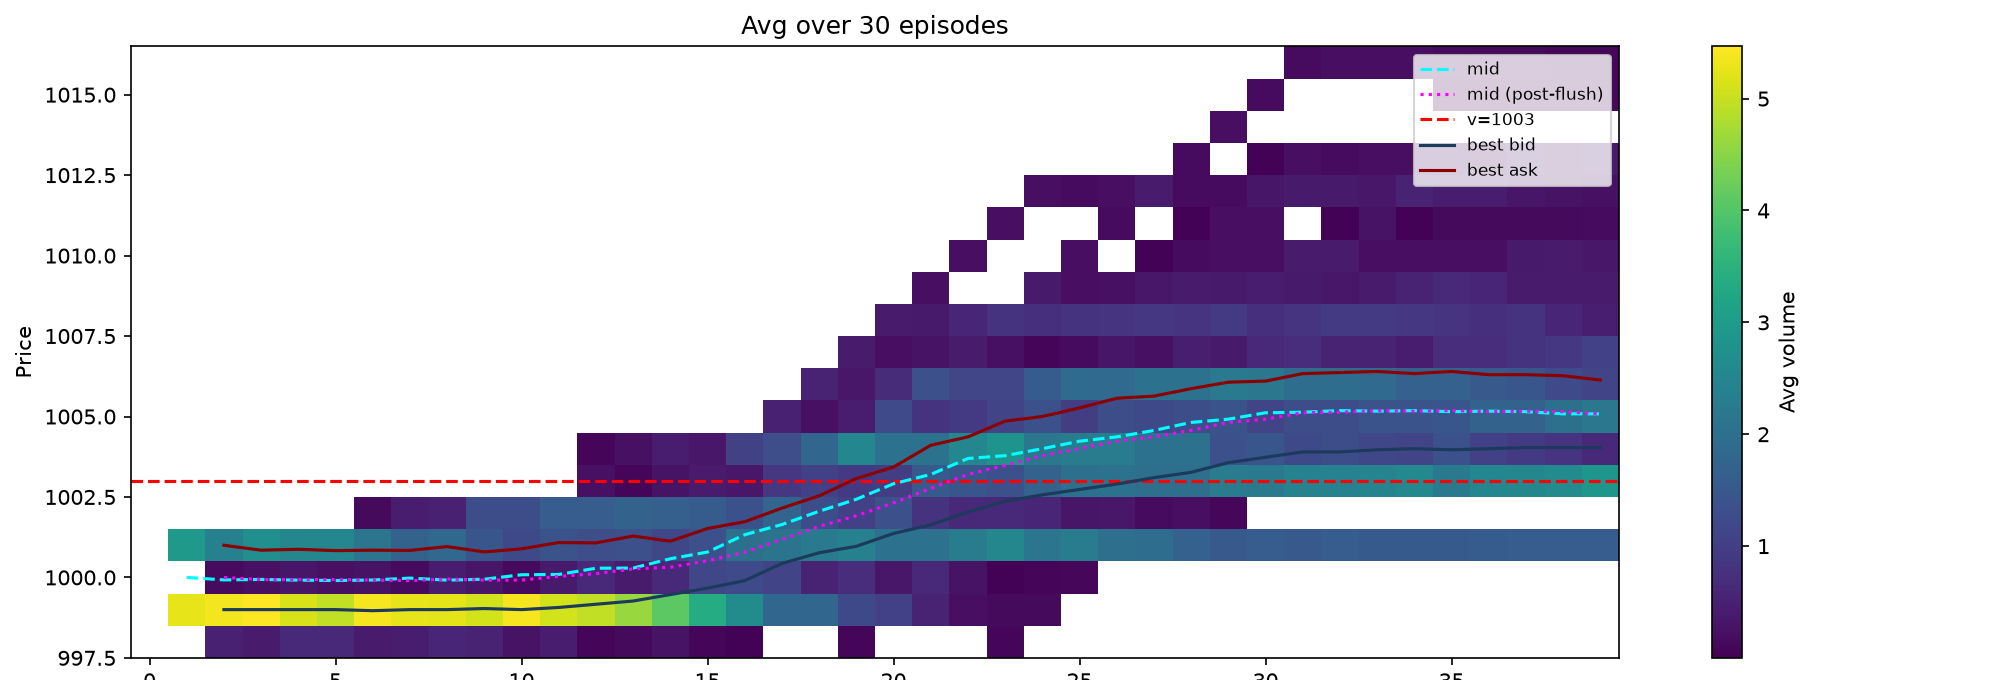
\includegraphics[width=\textwidth]{cropped/v1003_mixed_lob.png}
    \column{0.35\textwidth}
    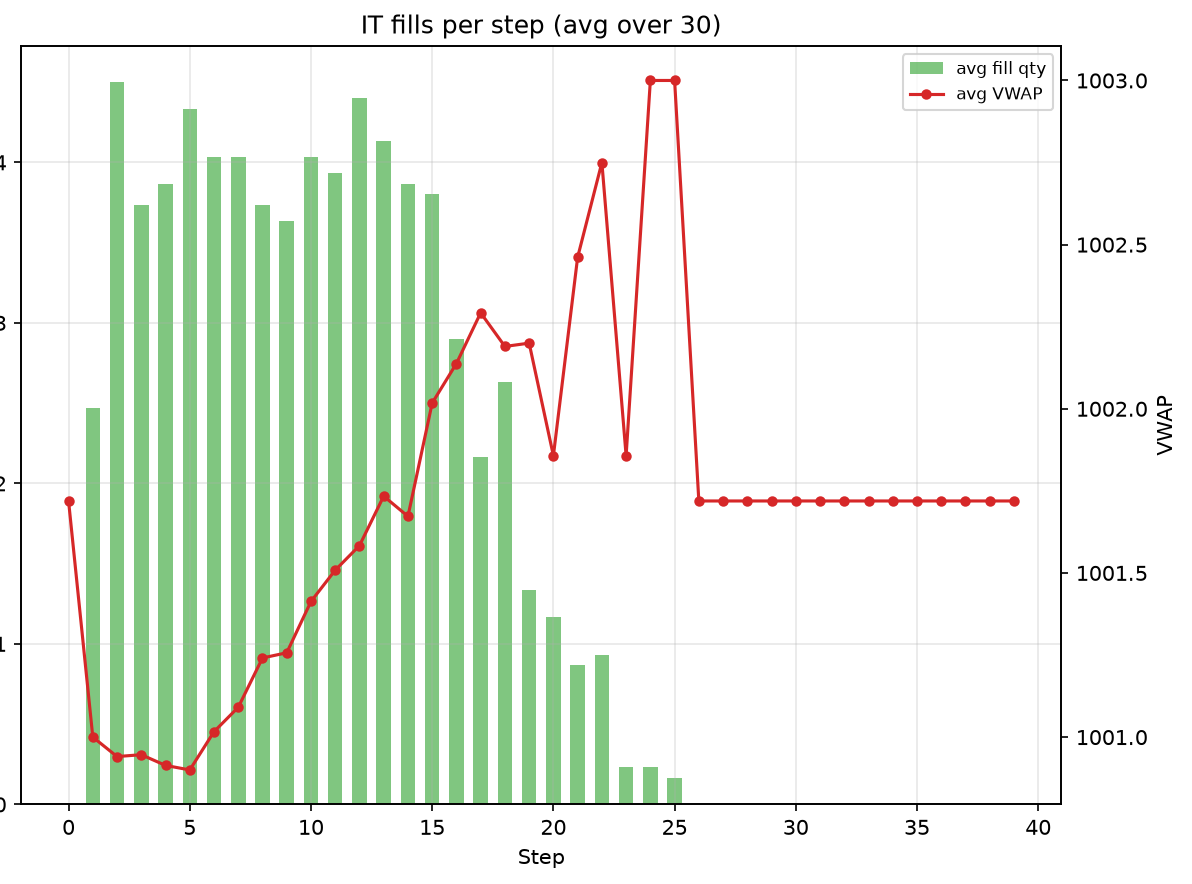
\includegraphics[width=\textwidth]{cropped/v1003_mixed_fills.png}
  \end{columns}
  \begin{itemize}
    \item Smooth convergence toward $v$ -- no dip, analytical HJB MMs anchor the mid
    \item PPO $\kappa$ converges steadily to $\sim 1.25$--$1.35$ over the episode
    \item IT $\beta$ oscillates $\sim 3$--$6$ -- higher than HJB-only due to more MM competition
  \end{itemize}
\end{frame}

\begin{frame}{$v = 1006$ -- HJB-Only (IT vs 5 analytical HJB MMs)}
  \begin{columns}[T]
    \column{0.62\textwidth}
    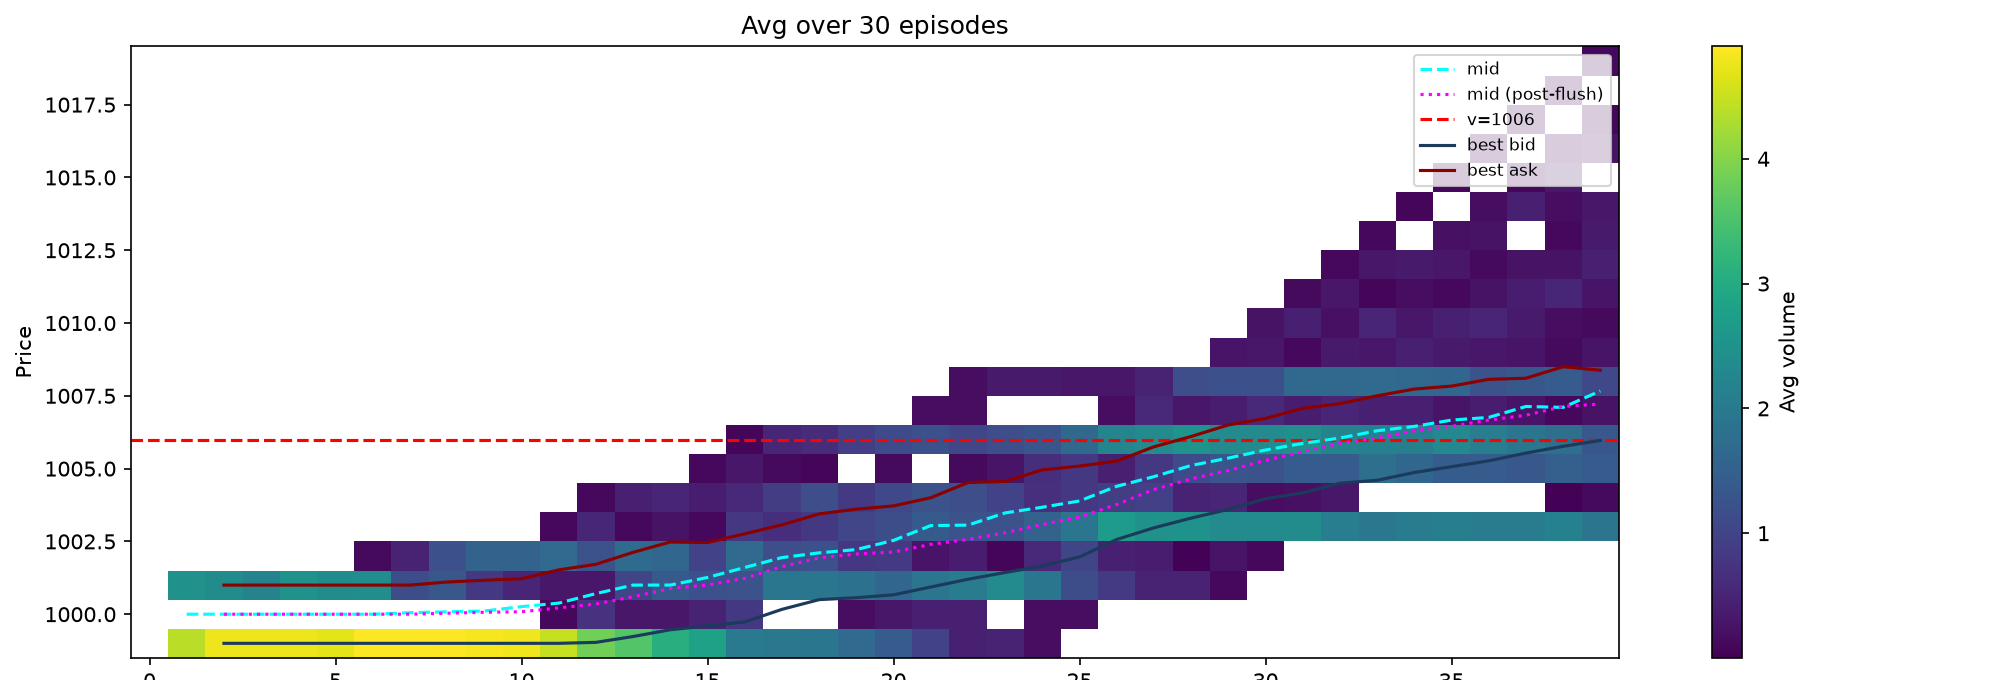
\includegraphics[width=\textwidth]{cropped/v1006_hjb_lob.png}
    \column{0.35\textwidth}
    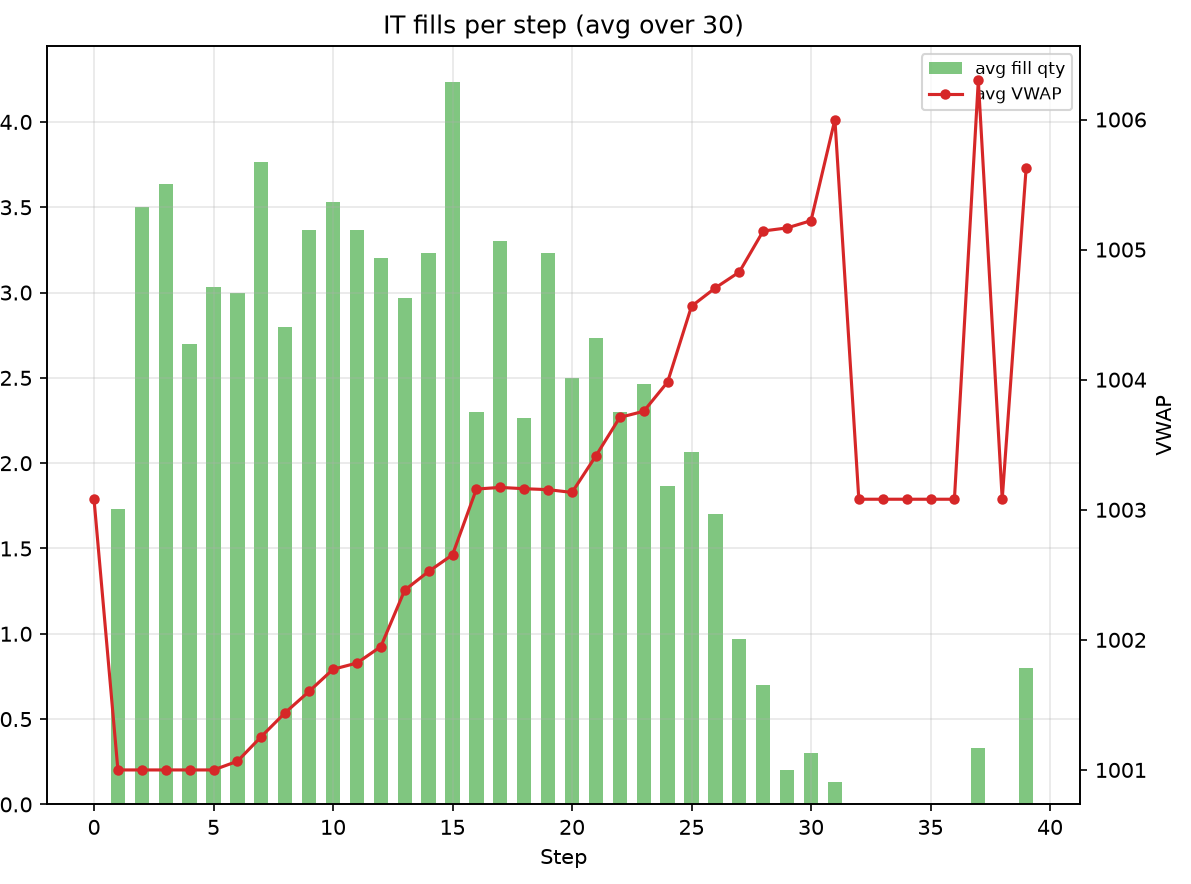
\includegraphics[width=\textwidth]{cropped/v1006_hjb_fills.png}
  \end{columns}
  \begin{itemize}
    \item Mid rises toward $v = 1006$, but ends $\sim 1004$ -- incomplete convergence within 40 steps
    \item IT $\beta$ oscillates $\sim 4$--$7$, consistently higher than the $v = 1003$ case
    \item Larger fair value gap $\rightarrow$ larger mispricing $\rightarrow$ more aggressive IT
  \end{itemize}
\end{frame}

\begin{frame}{$v = 1006$ -- PPO-Only (IT vs 5 PPO HJB MMs)}
  \begin{columns}[T]
    \column{0.62\textwidth}
    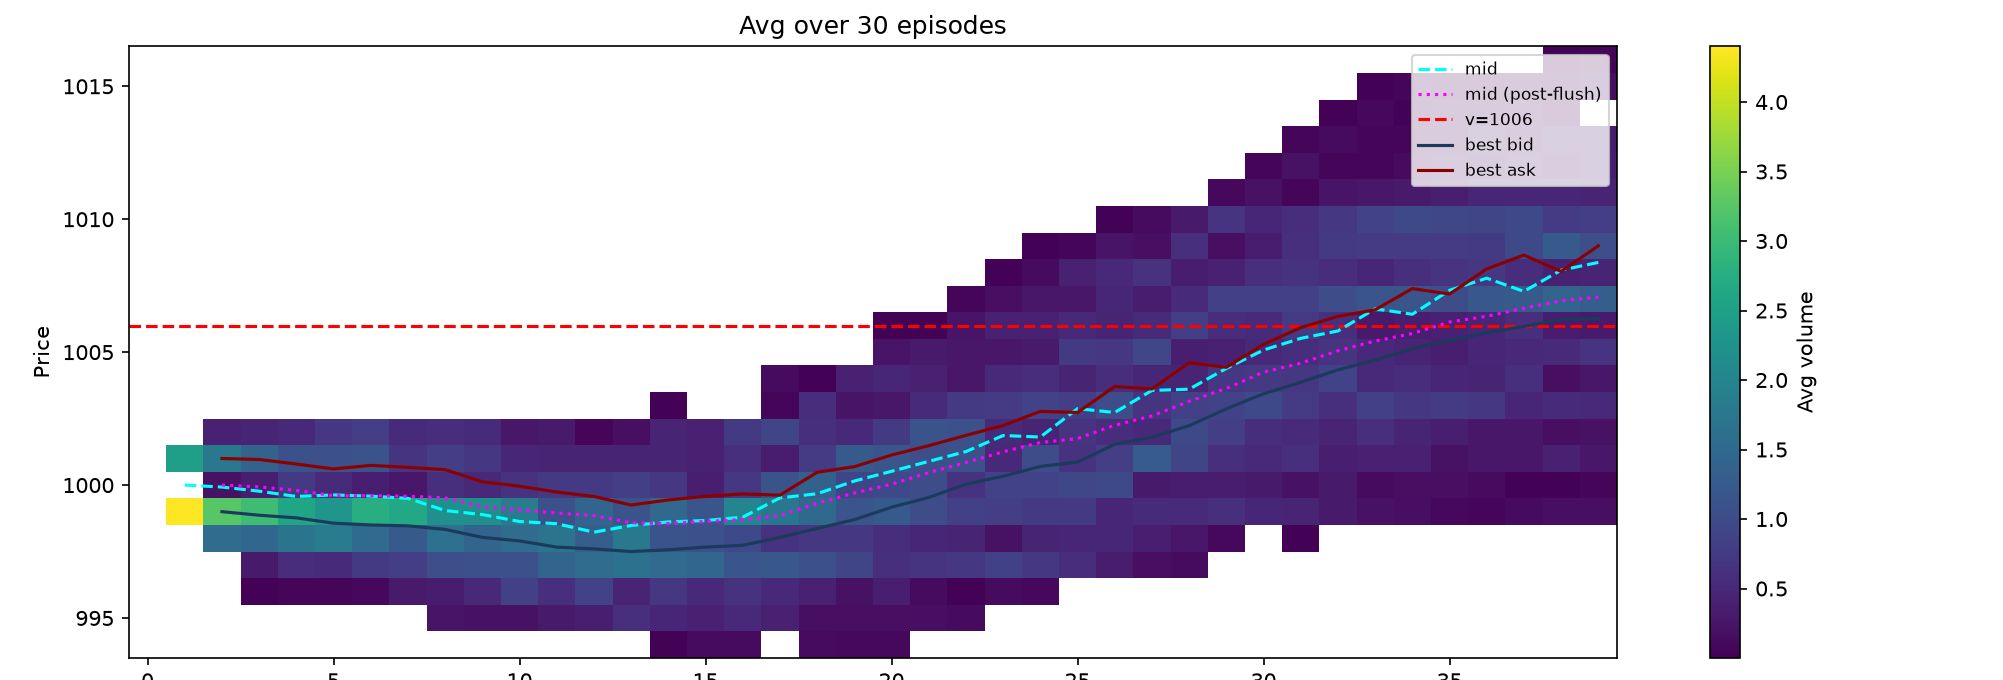
\includegraphics[width=\textwidth]{cropped/v1006_ppo_lob.png}
    \column{0.35\textwidth}
    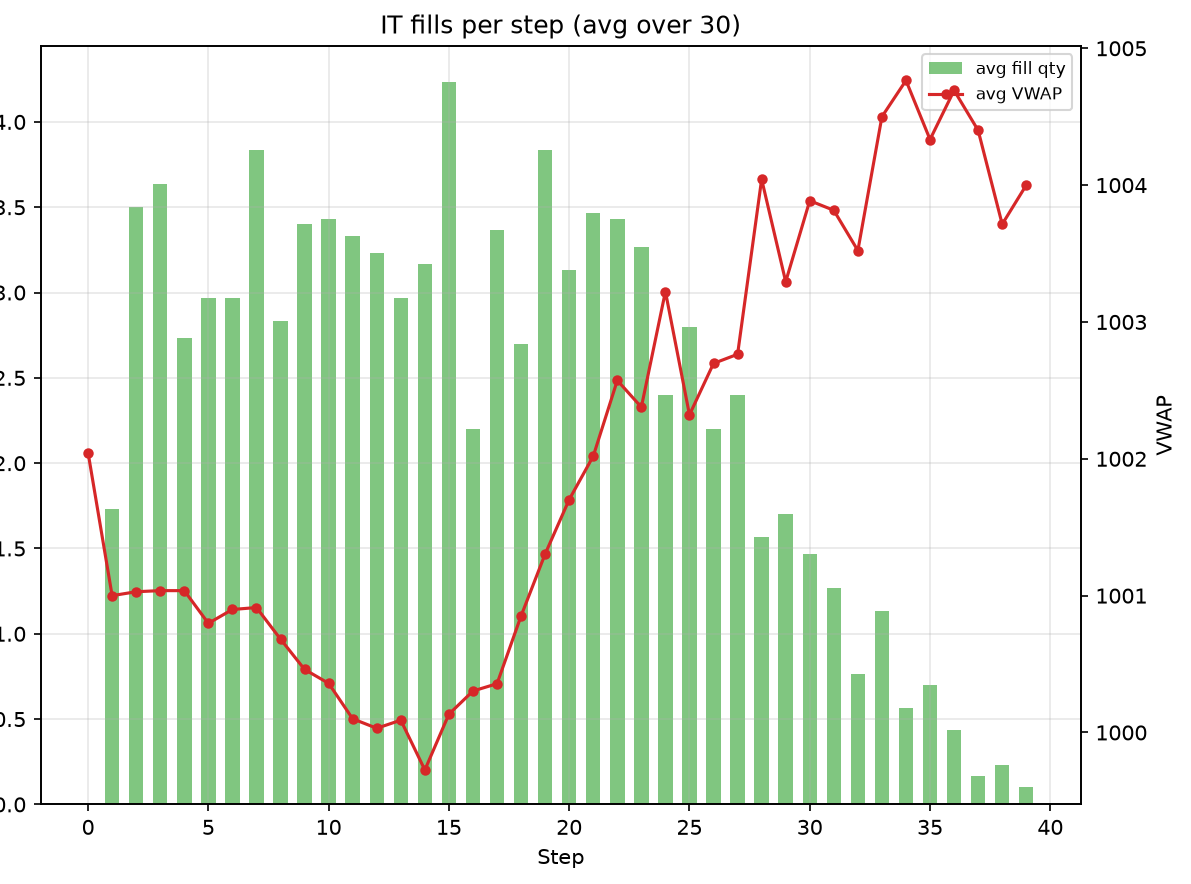
\includegraphics[width=\textwidth]{cropped/v1006_ppo_fills.png}
  \end{columns}
  \begin{itemize}
    \item Dip pattern observed but less pronounced than at $v = 1003$
    \item $\kappa$ stays high ($\sim 1.2$--$1.4$) -- MMs less reactive because IT demand is already priced in
    \item Mid ends $\sim 1004$--$1005$, about $1$--$2$ ticks below $v$
  \end{itemize}
\end{frame}

\begin{frame}{$v = 1006$ -- Mixed (IT vs 3 HJB + 3 PPO HJB MMs)}
  \begin{columns}[T]
    \column{0.62\textwidth}
    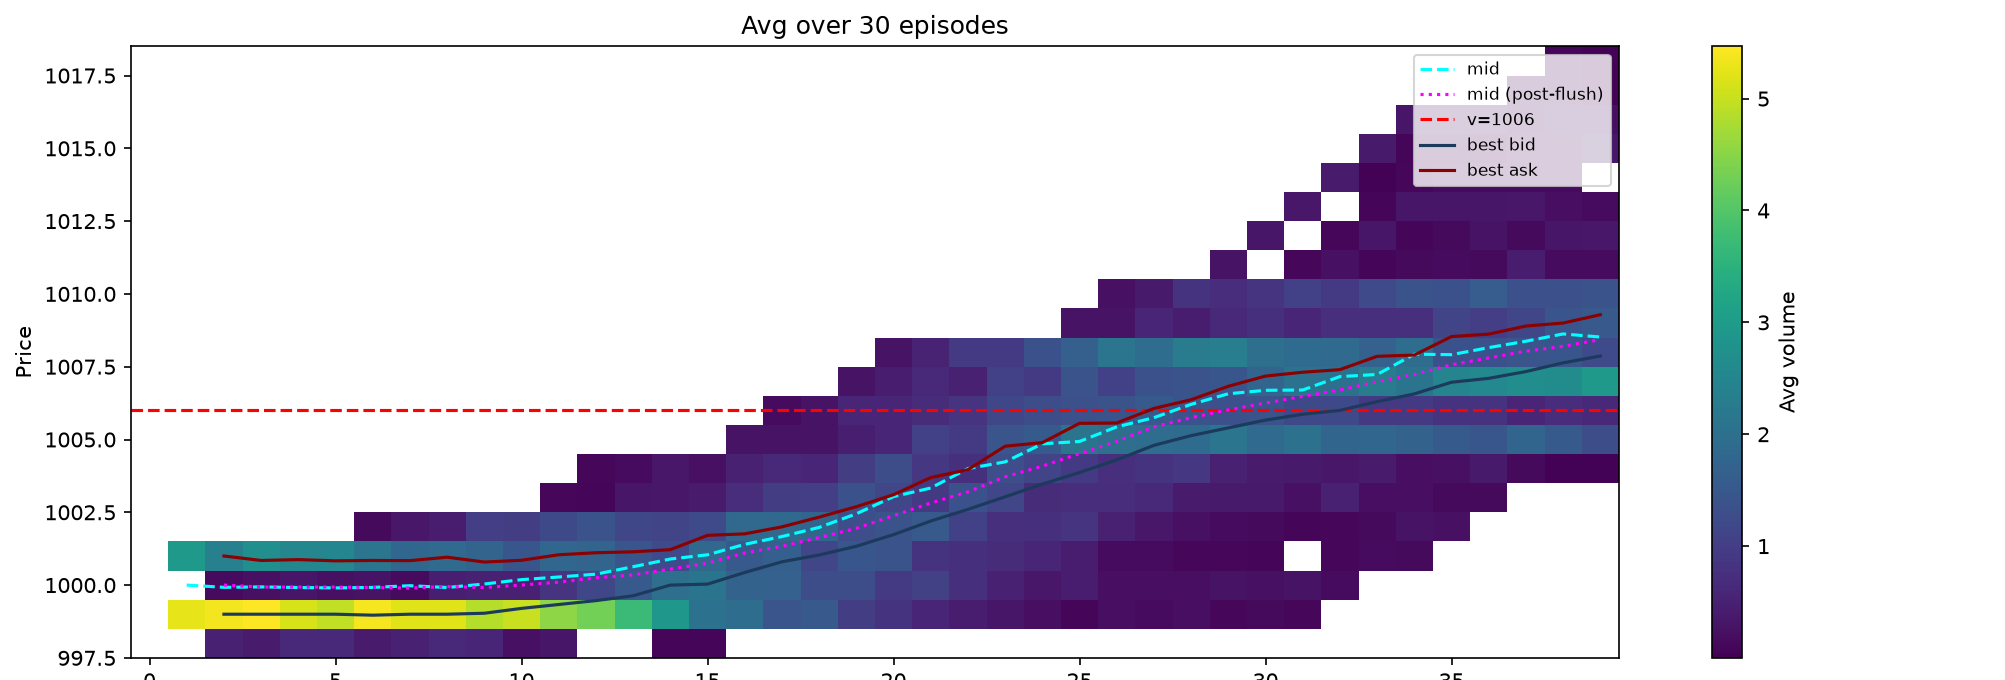
\includegraphics[width=\textwidth]{cropped/v1006_mixed_lob.png}
    \column{0.35\textwidth}
    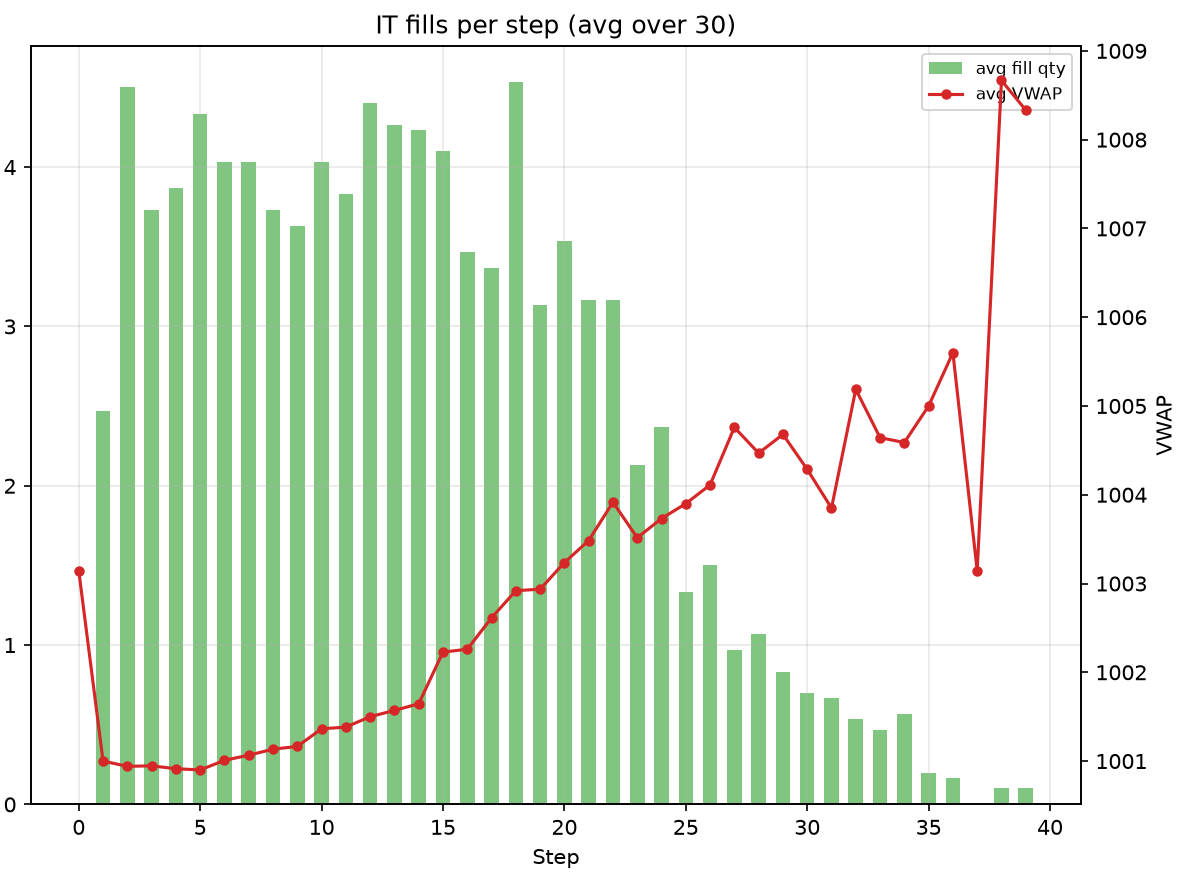
\includegraphics[width=\textwidth]{cropped/v1006_mixed_fills.png}
  \end{columns}
  \begin{itemize}
    \item Stable convergence, same pattern as the $v = 1003$ mixed case
    \item PPO $\kappa$ shows wider spread ($\sim 1.1$--$1.3$) than the $v = 1003$ case
    \item IT $\beta \sim 4$--$8$, the highest across all experiments (more MM targets = more trading)
  \end{itemize}
\end{frame}

% =====================================================================
\section{Cross-Experiment Comparison}
% =====================================================================

\begin{frame}{HJB vs PPO: Key Differences}
  \begin{columns}[T]
    \column{0.50\textwidth}
    \textbf{PPO-Only Behavior:}
    \begin{itemize}
      \item \textbf{Dip-then-rise} signature: mid drops below ref\_price before converging toward $v$
      \item $\kappa$ drops initially (widening spreads) then rises (tightening)
      \item Without analytical anchor, MMs' collective quoting determines mid fully
    \end{itemize}

    \column{0.50\textwidth}
    \textbf{Mixed Behavior:}
    \begin{itemize}
      \item Smooth convergence -- no dip
      \item Analytical HJB MMs ($\kappa = 0.8$) provide a fixed quoting baseline
      \item PPO MMs learn to quote slightly tighter ($\kappa > 1.0$) to compete
      \item IT can exploit both MM types -- higher $\beta$, more execution
    \end{itemize}
  \end{columns}

  \vspace{8pt}
  \begin{center}
  \begin{tabular}{lccc}
    \toprule
    Metric & HJB-Only & PPO-Only & Mixed (3+3) \\
    \midrule
    Mid convergence & Steady & Dip-then-rise & Smooth \\
    $\kappa$ range (PPO) & N/A & $1.07$--$1.32$ & $1.10$--$1.35$ \\
    IT $\beta$ (v=1003) & $2$--$3$ & $2$--$5$ & $3$--$6$ \\
    IT $\beta$ (v=1006) & $4$--$7$ & $3$--$7$ & $4$--$8$ \\
    \bottomrule
  \end{tabular}
  \end{center}
\end{frame}

\begin{frame}{Effect of Fair Value $v$}
  \begin{columns}[T]
    \column{0.48\textwidth}
    \centering
    \textbf{$v = 1003$ (3 ticks above ref)}
    \begin{itemize}
      \item Smaller mispricing signal
      \item IT moderates aggression ($\beta \sim 2$--$5$)
      \item Mid converges within $\sim 0.5$ ticks of $v$
      \item Clearer differentiation between MM types
    \end{itemize}

    \column{0.48\textwidth}
    \centering
    \textbf{$v = 1006$ (6 ticks above ref)}
    \begin{itemize}
      \item Larger mispricing $\rightarrow$ more aggressive IT
      \item IT $\beta$ reaches $7$--$8$ in mixed case
      \item Mid ends $1$--$2$ ticks below $v$ -- incomplete convergence within 40 steps
      \item MMs forced wider spreads to survive adverse selection
    \end{itemize}
  \end{columns}

  \vspace{6pt}
  \textbf{Takeaway:} Larger fair value gaps create stronger adverse selection pressure.
\end{frame}

\begin{frame}{The Dip-Then-Rise: Mechanism}
  \textbf{PPO-only: mid drops below ref\_price ($\sim 997$) before rising toward $v$ ($\sim 1002.5$).}

  \begin{enumerate}
    \item \textbf{Step 0:} PPO MMs start with $\kappa \approx 1.15$ (moderate spread). IT begins buying.
    \item \textbf{Steps 1--10:} MMs observe fills, $\lambda_{\text{est}}$ rises.
          They \textbf{lower $\kappa$ to $\approx 1.07$} (widen spread) as protection.
    \item \textbf{Asymmetric effect:} IT only hits the ask. No one hits the bid.
          $\rightarrow$ best bid drifts down, mid $\textbf{drops}$.
    \item \textbf{Steps 10--30:} $\lambda_{\text{est}}$ stabilizes, $h(q)$ inventory penalty
          already accounts for risk. MMs \textbf{raise $\kappa$ to $\approx 1.32$}.
    \item \textbf{Steps 30--40:} Tighter quoting + IT buying drives mid toward $v$.
  \end{enumerate}

  \textbf{Why not in mixed?} Analytical HJB MMs ($\kappa = 0.8$, symmetric) keep the bid anchored.
\end{frame}

% =====================================================================
\section{Conclusion}
% =====================================================================

\begin{frame}{Summary}
  \begin{enumerate}
    \item \textbf{PPO HJB MMs learn adaptive quoting} -- they widen spreads in response to adverse selection and tighten once risk is priced in.
    \item \textbf{The dip-then-rise pattern} emerges only in PPO-only environments where no analytical anchor exists.
    \item \textbf{Mixed environments} produce the smoothest convergence. Analytical MMs provide a quoting floor; PPO MMs learn to compete by quoting slightly tighter.
    \item \textbf{Fair value matters}: larger $v - p_0$ gaps amplify adverse selection, increasing IT aggression and slowing price discovery.
    \item \textbf{3+3 MMs} were sufficient -- earlier 5+5 experiments showed instability at $v = 1006$.
  \end{enumerate}
\end{frame}

% =====================================================================
\appendix
\section{Annex -- Full Plots}
% =====================================================================

\begin{frame}{Annex: $v = 1003$ -- HJB-Only}
  \begin{center}
    \includegraphics[width=0.45\textwidth]{../results_v1003_hjb/eval_avg.png}%
    \hfill
    \includegraphics[width=0.45\textwidth]{../results_v1003_hjb/beta_avg.png}
  \end{center}
\end{frame}

\begin{frame}{Annex: $v = 1003$ -- PPO-Only}
  \begin{center}
    \includegraphics[width=0.45\textwidth]{../results_v1003_ppo/eval_avg.png}%
    \hfill
    \includegraphics[width=0.45\textwidth]{../results_v1003_ppo/beta_avg.png}

    \vspace{4pt}
    \includegraphics[width=0.45\textwidth]{../results_v1003_ppo/ppo_hjb_avg.png}
  \end{center}
\end{frame}

\begin{frame}{Annex: $v = 1003$ -- Mixed (3+3)}
  \begin{center}
    \includegraphics[width=0.45\textwidth]{../results_v1003_mixed_3mms/eval_avg.png}%
    \hfill
    \includegraphics[width=0.45\textwidth]{../results_v1003_mixed_3mms/beta_avg.png}

    \vspace{4pt}
    \includegraphics[width=0.45\textwidth]{../results_v1003_mixed_3mms/ppo_hjb_avg.png}
  \end{center}
\end{frame}

\begin{frame}{Annex: $v = 1006$ -- HJB-Only}
  \begin{center}
    \includegraphics[width=0.45\textwidth]{../results_v1006_hjb/eval_avg.png}%
    \hfill
    \includegraphics[width=0.45\textwidth]{../results_v1006_hjb/beta_avg.png}
  \end{center}
\end{frame}

\begin{frame}{Annex: $v = 1006$ -- PPO-Only}
  \begin{center}
    \includegraphics[width=0.45\textwidth]{../results_v1006_ppo/eval_avg.png}%
    \hfill
    \includegraphics[width=0.45\textwidth]{../results_v1006_ppo/beta_avg.png}

    \vspace{4pt}
    \includegraphics[width=0.45\textwidth]{../results_v1006_ppo/ppo_hjb_avg.png}
  \end{center}
\end{frame}

\begin{frame}{Annex: $v = 1006$ -- Mixed (3+3)}
  \begin{center}
    \includegraphics[width=0.45\textwidth]{../results_v1006_mixed_3mms/eval_avg.png}%
    \hfill
    \includegraphics[width=0.45\textwidth]{../results_v1006_mixed_3mms/beta_avg.png}

    \vspace{4pt}
    \includegraphics[width=0.45\textwidth]{../results_v1006_mixed_3mms/ppo_hjb_avg.png}
  \end{center}
\end{frame}

\end{document}
